\chapter{Experimentation}
\label{ch_experimentation}
%This is a chapter added into the template because Dr. Winberg's example reports have it.

\section{Testing Methodology}

Testing was performed in two phases, the first phase involves testing of individual modules. This modular testing is analogous to unit-tests in the computer programming paradigm. The second phase of testing involves characterising the performance of the final system prototype.

\subsection{Focal Length of Lens}
\label{exp:focal_length}
To generate the beam of light from the IR LED, a light focusing tube was created with a lens as described in the design section. To determine the dimensions of the light focusing tube, the focal length of the lens needed to be measured.

Figure \ref{fig:focal_length_experiemnt} shows the experimental setup used to determine the focal length of the lens. The lens was secured to a pair of 'helping-hands' to allow for precise adjustment of height above the working surface. A light source was placed directly above the lens at a distance of 1.2m.

\begin{figure}[H]
		\centering
		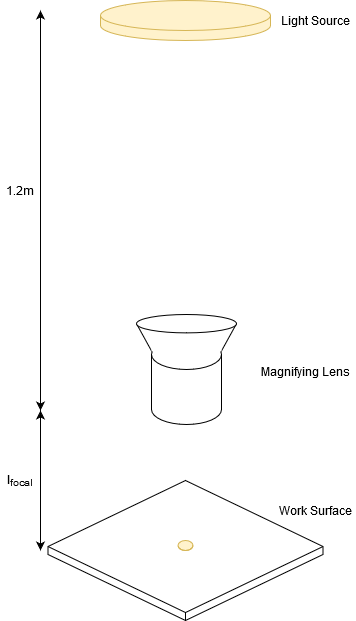
\includegraphics[width=.4\linewidth]{figures/experimentation/focal_length.png}
		\captionof{figure}{Focal Length Experiment Setup}
		\label{fig:focal_length_experiemnt}
\end{figure}

After setting up the experiment, the lens was slowly adjusted along the vertical until the spot formed on the work surface was a minimum. A tape measure was used to find the distance from the work surface to the lens.

\subsection{Light Focus System}

To test the light focusing tube, two power LEDs where used. Initially, a 3W warm white (visible light) power LED was used to confirm the functionality of the system. Following this, the 3W IR power LED was used.

In both cases, the focus system was setup a specific distance from a flat surface. The light was then powered and the edge of the beam spot was marked and the diameter taken. To determine the location of the IR beam spot edge, a video camera in 'night shot' mode was used.

\begin{figure}[H]
	\centering
	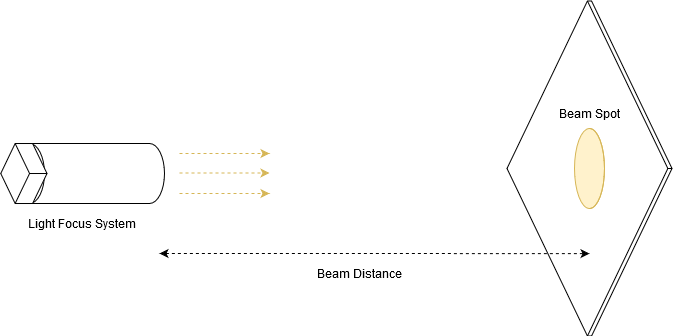
\includegraphics[width=.7\linewidth]{figures/experimentation/beam_spot_experiement.png}
	\captionof{figure}{Light Focus System Experiment Setup}
	\label{fig:focus_system_experiemnt}
\end{figure}

%todo: Give distances for measuredments taken
Figure \ref{fig:focus_system_experiemnt} above shows the experimental setup. The experiment was performed for distances of x, y, z.

\subsection{Goertzel Filter Optimization}

To understand the benefits to be gained from optimization and to understand the effectiveness of the two optimization methods the following experiment were performed to give insight into the effect of increasing the number of samples (N) and optimizing the algorithm by reducing the number of multiplications.

First, the goertzel algorithm as given in listing \ref{lst:goertzel_algorithm} was converted to C and implemented inside the circular buffer's callback functions. This implementation is referred to as the unoptimized algorithm. As a consequence of using a circular buffer with two segments, there are two callback functions. The goertzel implementation inside both callback functions were the same, with the only exception being the location in the buffer from which samples were read.

The timing was measured externally using an oscilloscope, to achieve this, just before the goertzel algorithm began executing an LED was turned on using one of the GPIO pins. This LED was turned off as soon as the algorithm finished calculating the result. Each of the two callback functions used a unique GPIO pin to toggle separate LEDs. Figure \ref{fig:goertzel_optimization_experiemnt} below illustrates the experimental setup in the form of a block diagram.

\begin{figure}[H]
	\centering
	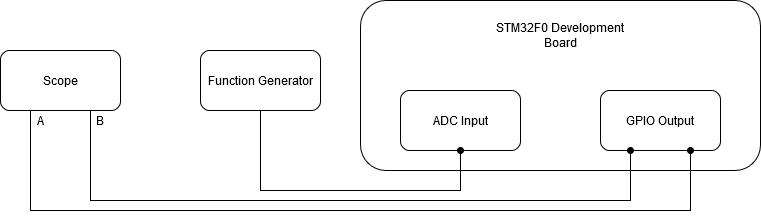
\includegraphics[width=.9\linewidth]{figures/experimentation/goertzel_speed_test_diagram.png}
	\captionof{figure}{Goertzel Optimization Experimental Setup}
	\label{fig:goertzel_optimization_experiemnt}
\end{figure}

A signal generator was used to produce a 36kHz sine waveform with an amplitude of 1V and an offset of 1V. Using a signal generator ensured that a known waveform was present at the input to the goertzel filter, in addition, by using a 36kHz waveform the filter is forced to deal large sample values which gives insight into performance under the most demanding circumstances.

The experiment was broken into iterations, each iteration began by setting N to the desired number of samples, following this the code was compiled and executed on the development board. The signal generator was attached and enabled and the scope probes were attached to the GPIO pins responsible for indicating timing. The scope was then adjusted so that between 20 and 30 pulses could be seen. 

The independent variable N (number of samples to process) was set to 4 for the first iteration and doubled for each consecutive iteration until a value of 64 was reached. These five values of N were chosen because they preserve the ratio given in equation \ref{eqn:k_N_and_fb_fs_ratio} which is a requirement for the optimization to work.

Using the measurement tools built into the Picoscope software the 'high pulse width' for both GPIO pin outputs was measured, along with the duty cycle of those waveforms. The average of all pulses was recorded.

For the purposes of this experiment only the 'high pulse width' of the callback responsible for the first half of the circular buffer being full was necessary to draw conclusions regarding the algorithms performance. The timing for the second half of the buffer being full was used only as a sanity check, both the callback functions should run for the same amount of time as each is executing the same algorithm therefore the average high pulse width for each should be the same.

After the experiment was run for all 5 iterations, the goertzel implementation was modified by removing the unnecessary multiplications (as discussed in section \ref{sec:filter_optimization_design}) and the above experiment repeated following the same method.


%Filter performance experiment:
% - Impact of multiplication in algorithm
% - Impact of N


\subsection{Goertzel Filter Performance}

To evaluate the performance of the goertzel filter the following experiments where performed.

\begin{itemize}
	\item Simulated Frequency Response
	\item Measured Frequency Response
	\item Trigger Conditions
\end{itemize}

\subsubsection{Simulated Frequency Response}
The expected frequency response was determined using the Octave\footnote{Open-source alternative to Matlab} environment. This was achieved by first creating a goertzel filter with the exact same optimized algorithm as the one implemented on the STM32 and a main script to interface with the function. The octave Goertzel function is given in listing \ref{lst:optimized_goertzel_algorithm}. This function is optimized according to the design outlined in section \ref{sec:filter_optimization_design} and the value returned by the function is the magnitude of the DFT coefficient squared.

Following this the interface Octave script was written to find the filter response (see listing \ref{lst:frequency_response_script}). This script generated a range of frequencies in the form of sampled sin waves over the range of 0Hz to 71.7kHz with an interval of 100Hz. To simulate the behaviour of the filter, the test frequencies were scaled, off-set and sampled to match the expected conversion values returned by the ADC. After generating each frequency, the above mentioned octave implementation of the Goertzel filter was called and the computation result stored. An example, 36kHz waveform is given in the appendix, figure \ref{fig:sampled_36khz_sinusoid}.

The frequency response was plotted to provide an insight into the expected performance of the digital filter. The frequency response was tested with sinusoids of amplitude 1V and again with sinusoids of amplitude 500mV.

\subsubsection{Measured Frequency Response}
The next experiment involved testing the Goertzel filter to check that the filter implementation was working as expected. This was done by generating a sinusoid waveform at the input to the ADC and using the serial communication port to transfer the value of the Goertzel filtering result. 

The experimentation was performed on the STM32 development board. This process involved manually configuring the function generator for each individual frequency and then pushing a button on the development board to transfer the most recent filter result.

The first frequency tested was 1kHz, this frequency was incremented by 3kHz per reading until a frequency of 70kHz was reached. The results were processed by Octave to generate a plot and compare the empirical results with the simulated response.


\subsubsection{Trigger Conditions}
%Trigger Frequency vs amplitude | Trigger frequency
To test the high-level functionality of the Goertzel

















\newpage
\subsection{Tests $\setminus$ Results to gather}

\textbf{Hardware}
\begin{itemize}
	\item IR Power LED:
	\begin{itemize}
		\item Beam angle (focus vs no focus)
		\item Beam strength (LUX)
		\item LED Current draw
		\item LED temperature (basic sensor or a temperature gun that I borrow from somewhere)
		\item MOSFET temperature
	\end{itemize}
	\item For each photo-sensor (photodiode, phototransistor, all in one receiver module):
	\begin{itemize}
		\item Receiving beam-angle
		\item Output signal strength vs light-intensity/distance
		\item Reaction time (rise time)
		\item multipath/picking up reflections
		\item Signal to noise ration
	\end{itemize}
	\item Op-Amp:
	\begin{itemize}
		\item Op-amp gain performance (push to limit) (at 36kHz)
		\item Op-amp frequency performance (at some fixed gain)
		\item Filter performance (anti-aliasing and high pass filtering)
	\end{itemize}

	\item compare different frequencies to determine if interference causes any issues...
\end{itemize}

\textbf{Software}
\begin{itemize}
	
	\item Transmitter
	\begin{itemize}
		\item Timing accuracy
	\end{itemize}
	
	%\item Protocol
	%\begin{itemize}
	%	\item
	%\end{itemize}
	
	\item Receiver
	\begin{itemize}
		\item Bit error rate / max receiver distance - (not sure how I will implement this yet)
		\item Bit error correction - (not sure how I might implement this yet)
		\item Modulation to High/Low logic value [DSP processing analysis]
		\begin{itemize}
			\item Latency
			\item Testing the timing between stages of demodulating and decoding
		\end{itemize}
	\end{itemize}
	
\end{itemize}